\subsubsection{UC1}
\label{sub:uc1}

%TODO aggiornare caption con nome più preciso
\begin{figure}[h]
    \centering
    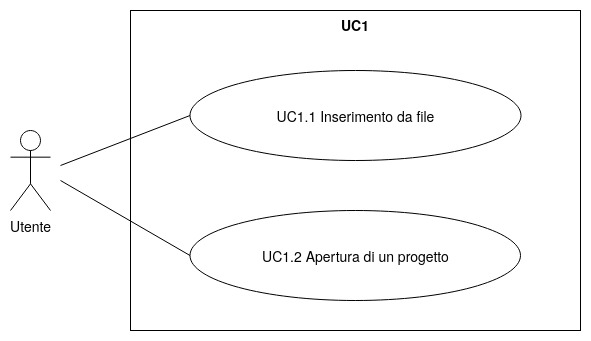
\includegraphics[width=0.5\textwidth]{componenti/casi-duso/diagrammi/UC1.jpg}
    \caption{UC1 - }
    \label{fig:UC1}
\end{figure}


\begin{itemize}
    \item{\textbf{Descrizione}}: L'utente effettua l'inserimento dei dati da elaborare;
    \item{\textbf{Attore primario}}: Utente;
    \item{\textbf{Attori secondari}}: Database;
    \item{\textbf{Precondizione}}: L'utente possiede un file contenente i dati da importare, o esiste un DB da dove recuperarli o ha già salvato un progetto precedente;
    \item{\textbf{Postcondizione}}: I dati o il progetto vengono importati in HD Viz;
    \item{\textbf{Scenario principale}}:
    \begin{enumerate}
        \item L'utente apre l'applicativo;
        \item All'utente viene proposto di importare un file contenente i dati, di scaricare i dati da una fonte esterna o di aprire un vecchio progetto;
        \item L'utente seleziona l'opzione desiderata;
        \item I dati o il progetto vengono importati all'interno di HD Viz.
    \end{enumerate}
\end{itemize}

\subsection{UC 1.1: inserimento dei dati tramite file}
\begin{itemize}
    \item{\textbf{Descrizione}}: L'utente effettua l'inserimento dei dati da elaborare mediante file .csv;
    \item{\textbf{Attore primario}}: Utente;
    \item{\textbf{Precondizione}}: L'utente possiede un file .csv contenente i dati da importare;
    \item{\textbf{Postcondizione}}: I dati vengono importati in HD Viz;
    \item{\textbf{Scenario principale}}: L'utente seleziona il file .csv da importare;
\end{itemize}

\subsection{UC 1.2: apertura di un progetto precedente}
\begin{itemize}
    \item{\textbf{Descrizione}}: L'utente effettua l'inserimento dei dati da elaborare;
    \item{\textbf{Attore primario}}: Utente;
    \item{\textbf{Precondizione}}: L'utente possiede un progetto precedente;
    \item{\textbf{Postcondizione}}: Il progetto viene importato in HD Viz;
    \item{\textbf{Scenario principale}}: All'utente vengono presentati i progetti precedentemente creati. L'utente, una volta scelto quello desiderato, dovrà poter riprendere l'esplorazione dei dati da dove l'aveva lasciata.
\end{itemize}

\subsection{UC 1.3: Inserimento da database}
\begin{itemize}
    \item{\textbf{Descrizione}}: L'utente effettua l'inserimento dei dati da elaborare;
    \item{\textbf{Attore primario}}: Utente;
    \item{\textbf{Attori secondari}}: Database contenente i dati;
    \item{\textbf{Precondizione}}: Il database in oggetto contiene i dati da elaborare;
    \item{\textbf{Postcondizione}}: I dati vengono importati in HD Viz;
    \item{\textbf{Scenario principale}}: L'utente importa in HD Viz dei dati contenuti su un DB esterno.
\end{itemize}
